\documentclass[a4paper]{scrartcl}
\usepackage[utf8]{inputenc}
\usepackage[ngerman]{babel}
%\usepackage[usenames,dvipsnames,svgnames,table]{xcolor}
\definecolor{blau}{rgb}{0,0,0.75}         
\definecolor{orange}{rgb}{0.8,0.3,0}      
\usepackage{hyperref}
\hypersetup{
 pdftitle = {\LaTeX-Klassen und Pakete für den Einsatz im Bereich der Schule},
 pdfsubject = {},
 pdfauthor = {Johannes Pieper, Johannes Kuhaupt, Ludger Humbert, Andr\'e Hilbig},
 colorlinks = true,
 hypertexnames = true,
 linkcolor=blau, %
 filecolor=orange, %
 citecolor=blau,
 menucolor=orange, %
 urlcolor=orange,
 breaklinks=true
}
\usepackage{caption,xparse,xargs}
\usepackage[german=guillemets]{csquotes}
\usepackage{schule,syntaxdi,schulinf,schulphy}
\usepackage{placeins,float,prettyref}
\usepackage{newfloat}

\lstset{  %
	language=[LaTeX]TeX,                 % the language of the code
	basicstyle=\small,            % the size of the fonts that are used for the code
	numbers=left,                    % where to put the line-numbers
	numberstyle=\footnotesize,           % the size of the fonts that are used for the line-numbers
	stepnumber=2,                    % the step between two line-numbers. If it's 1, each line will be numbered
	numbersep=5pt,                   % how far the line-numbers are from the code
	backgroundcolor=\color{white},       % choose the background color. You must add \usepackage{color}
	showspaces=false,                % show spaces adding particular underscores
	showstringspaces=false,          % underline spaces within strings
	showtabs=false,                  % show tabs within strings adding particular underscores
	frame=false,                    % adds a frame around the code
	tabsize=2,                       % sets default tabsize to 2 spaces
	resetmargins=true,
	captionpos=b,                    % sets the caption-position to bottom
	title=,                    % show the filename of files included with \lstinputlisting;
	breaklines=true,
	breakautoindent=true,
	prebreak=\mbox{ $\curvearrowright$},
	postbreak=\mbox{$\rightsquigarrow$ },
	linewidth=\columnwidth,
	breakatwhitespace=true,         % sets if automatic breaks should only happen at whitespace 
	numberstyle=\tiny\color{gray},         % line number style
	keywordstyle=\color{blue},           % keyword style
	commentstyle=\color{OliveGreen},        % comment style
	stringstyle=\color{mauve},          % string literal style
	morekeywords={
	zeitpunkt, punkteitem, scaleSequenzdiagramm, newthread, newthreadtwo, 
	newinst, node, chainin, draw, to, dokName, jahrgang, minisec, subsection, 
	glqq, grqq, euro
}                % if you want to add more keywords to the set
}
\newcommand{\materialsammlung}{\url{http://ddi.uni-wuppertal.de/material/materialsammlung/index.html}}

\usepackage{pdfpages}
\begin{document}
 \thispagestyle{empty}
 \section*{Musterhafter Aufbau des Unterrichtsprüfungsentwurf}
 \begin{lstlisting}[gobble=0,multicols=2,basicstyle=\normalsize,caption={}]
\documentclass[
		a4paper,11pt,
		oneside,neuePO]
	{schuleub}
\usepackage[utf8]{inputenc}

\thema{Mein Besuchsthema}
\reihe{Reihe zum Test}
\seminarinfo{Seminar für das 
	Lehramt an Gymnasien und 
	Gesamtschulen}
\seminaradresse{Teststr.~24, 
	58\,035 Wursthausen}
\ort{Wursthausen}
\besuchtitel{Lustiger Besuch}
\lerngruppe[EF]{
		Einführungsphase}
\datum{20.04.2024}
\zeit{08:00}{10:00}
\stunde{1}
\schule{Traumgymnasium}
\raum{B 224}

\weiblich{20}
\maennlich{10}
\foerderbedarf{2}

\referendar{Willi Wuster}

\ausbildungsl{Müller}
\foerderbedarfl{Sarbina}{
		Simons}{Sehen}
\ako{Meier}[in]
\schulleiter{Humboldt}
\hauptseminar{Lagrange}

\fachEins{Informatik}{
		Torvalds}
\fachZwei{Chinesisch}{
		Xianxu}

\vorsitz{Newton}[r]
		 % Frau Newton: \vorsitz{Newton}
\schulvertreter{Einstein}
\fremderseminar{Knuth}[in]
\bekannterseminar{Turing}

\begin{document}
	\begin{teila}
		\subsection{Erster Punkt}
			\begin{stundenverlauf}
			 \zeitpunkt{10:30 Uhr} 
			 Einstieg & Vortrag &
			 	LV & Tafel \\ \hline
			 \zeitpunkt{10:38 Uhr} 
			 \ldots{} & weiter im 
			 Verlauf der Stunde & 
			 	EA & \\ \hline
			\end{stundenverlauf}
	\end{teila}
	
	\begin{teilb}
		\subsection{Erster Punkt}
	\end{teilb}
		
	\addsec{
		Literaturverzeichnis}
		
	\begin{anhang}
	 \externesDokumentMehrseitig
		{ab.pdf}
	\end{anhang}
	 \end{lstlisting}
\clearpage
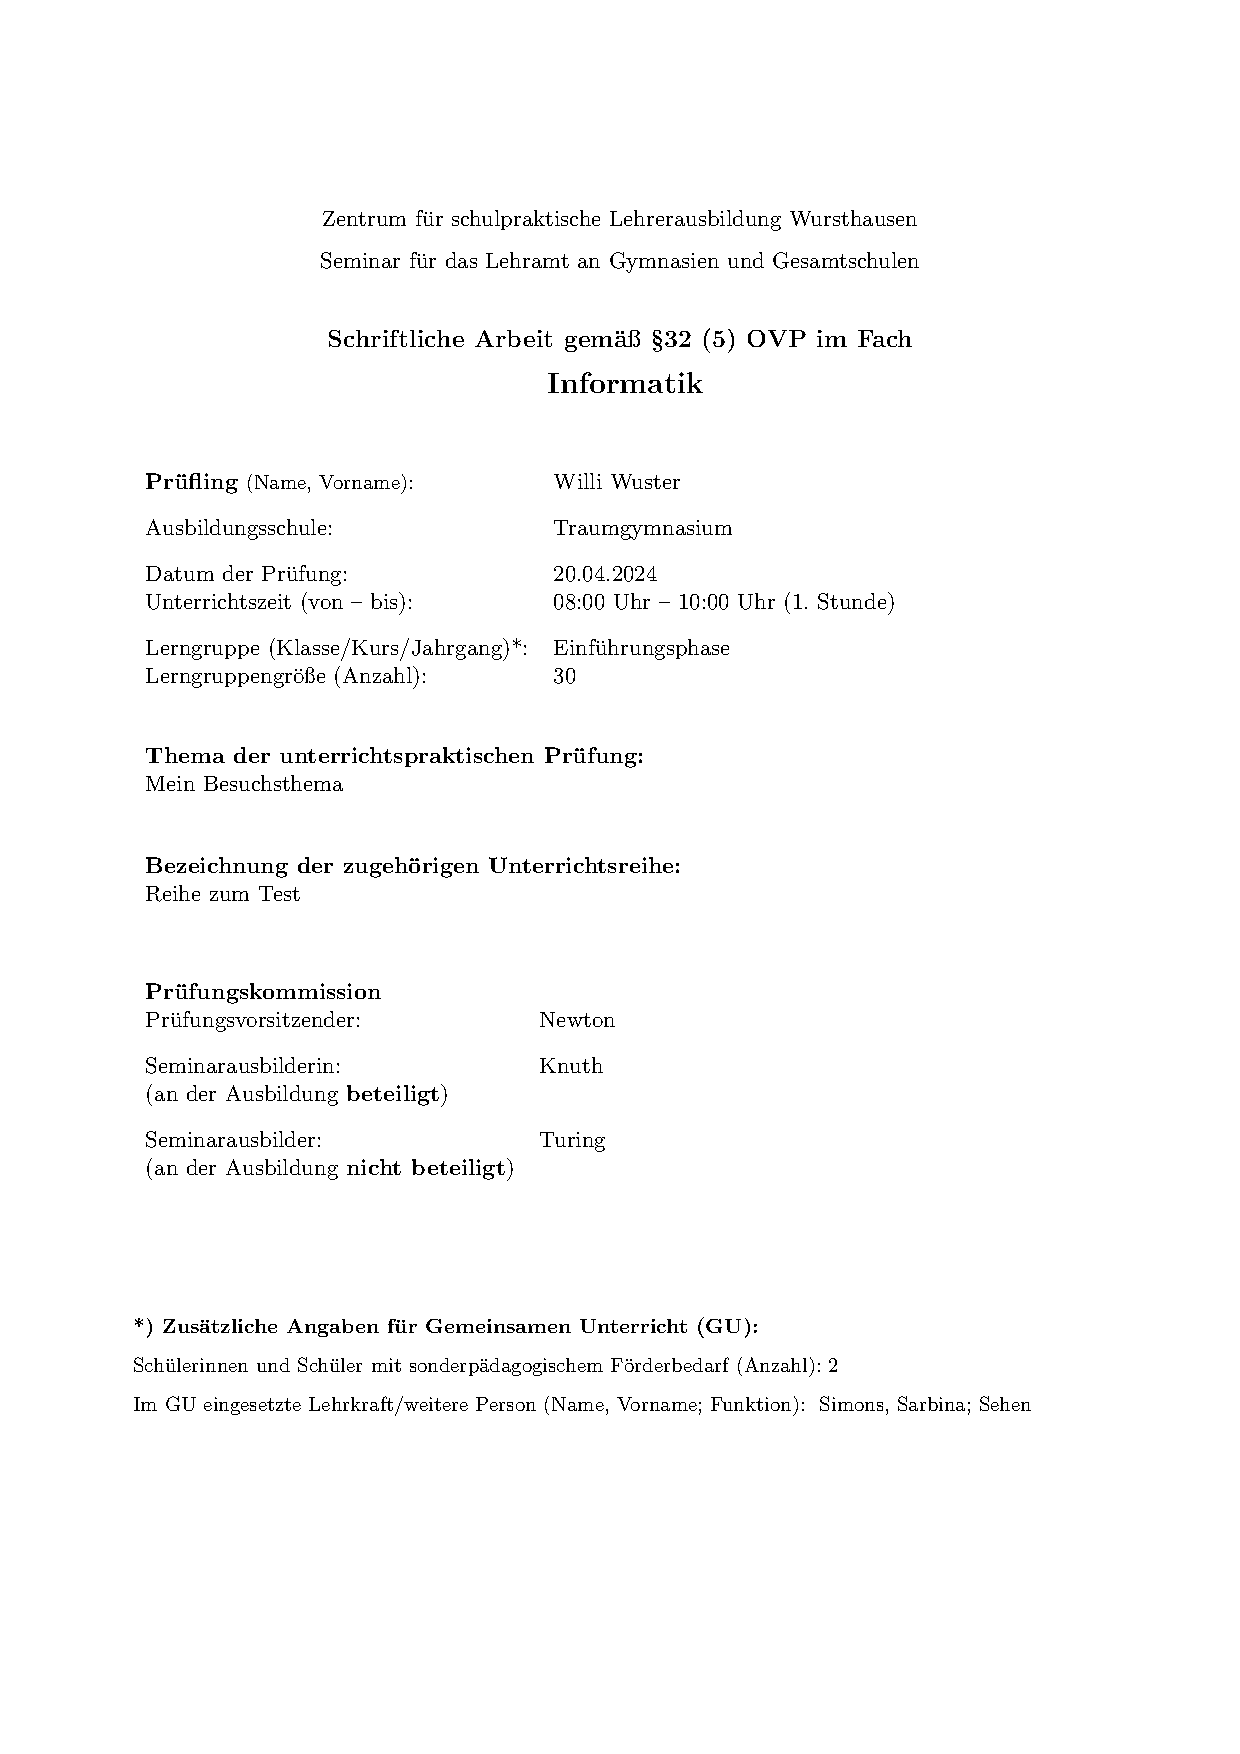
\includepdf[pages=1-last]{ub.pdf}
\end{document}
